\documentclass[chaptersright]{informeutn}
\usepackage[utf8]{inputenc}
\usepackage{array}
\usepackage{geometry}
\usepackage[table]{xcolor}
\usepackage{colortbl}
\usepackage{caption}
\usepackage{graphicx}
\usepackage{amsmath}
\usepackage{multirow}
\usepackage{float}
\usepackage{pgfplots}
\usepackage{pdfpages}

\pgfplotsset{compat=newest}


\materia{Dispositivos Electronicos I}
\titulo{Trabajo Practico N°4: JFET}
\comision{3R2}
\autores{Documentador y operador: Angelo Prieto 401012\\ Coordinador: Gaston Grasso 401892}
\fecha{16-09-2025}

\begin{document}
\maketitle
\tableofcontents

\chapter{Introduccion}
En este trabajo práctico se estudia el comportamiento de un transistor JFET de canal N. El objetivo 
principal es analizar sus características fundamentales tanto de manera teórica y mediante 
simulación, como a través de mediciones experimentales en el laboratorio.

A lo largo del desarrollo, se estudian parámetros esenciales como la corriente de saturación 
$I_{DSS}$, las características de salida y de transferencia, así como el fenómeno de estrangulamiento 
del canal. Para ello, primero se realizan simulaciones que permiten predecir el funcionamiento del 
dispositivo bajo diferentes condiciones de polarización. Posteriormente, se llevan a cabo mediciones 
experimentales con el fin de contrastar los resultados obtenidos.

En todo momento se tiene en cuenta la hoja de datos del dispositivo, a fin de permanecer dentro de 
los rangos de operación permisibles y evitar daños en el componente.


\chapter{Corriente de saturación}

    \section{Actividad de simulación}
    \begin{figure}[ht!]
        \centering
        \includegraphics[width=0.8\linewidth]{pictures/saturacion.png}
        \caption{circuito simulado en LTSpice.}
        \label{fig:sim-saturacion}
    \end{figure}
    
    \begin{figure}[ht!]
        \centering
        \includegraphics[width=0.8\linewidth]{pictures/graf-saturacion.png}
        \caption{gráfica de simulación $I_D=f(V_{DS})$}
        \label{fig:graf-saturacion}
    \end{figure}

Se puede observar en la gráfica obtenida de la simulación que la corriente de saturación
$I_{DSS} \approx 2.2mA$, para un valor de $V_{DS} \ge 1.4V$. Esto se corresponde con la hoja
de datos del dispositivo, en la cual se tiene la siguiente información:

\begin{table}[H]
    \centering
    \begin{tabular}{|c| c c c |c|}
        \hline
        Symbol & Min & Typ & Max & Unit\\
        \hline
        $I_{DSS}$ & 1.0 & 3.0  & 5.0 & mAdc    \\
        \hline
    \end{tabular}
    \caption{magnitud de $I_{DSS}$ sacado del datasheet.}
\end{table}
    
\section{Actividad de laboratorio}
\begin{table}[h!]
    \centering
    \begin{minipage}{0.45\textwidth}
        \centering
        \begin{tabular}{c c c}
            \toprule
            $V_{DD}$ [V] & $V_{DS}$ [V] & $I_{DS}$ [mA] \\
            \midrule
            0     & 0  & 0    \\
            5.96  & 1  & 1    \\
            7.72  & 2  & 1.27 \\
            9.46  & 3  & 1.31 \\
            10.93 & 4  & 1.42 \\
            12.43 & 5  & 1.52 \\
            13.89 & 6  & 1.62 \\
            15.43 & 7  & 1.72 \\
            \bottomrule
        \end{tabular}
    \end{minipage}%
    \hfill
    \begin{minipage}{0.45\textwidth}
        \centering
        \begin{tabular}{c c c}
            \toprule
            $V_{DD}$ [V] & $V_{DS}$ [V] & $I_{DS}$ [mA] \\
            \midrule
            16.97 & 8  & 1.87 \\
            18.3  & 9  & 1.91 \\
            19.7  & 10 & 1.99 \\
            21.2  & 11 & 2.08 \\
            22.6  & 12 & 2.18 \\
            24.2  & 13 & 2.30 \\
            25.8  & 14 & 2.41 \\
            27.3  & 15 & 2.61 \\
            \bottomrule
        \end{tabular}
    \end{minipage}
    \caption{Valores medidos de $I_{DS} = f(V_{DS})$.}
\end{table}


\begin{figure}[h!]
    \centering
    \resizebox{0.75\textwidth}{!}{
    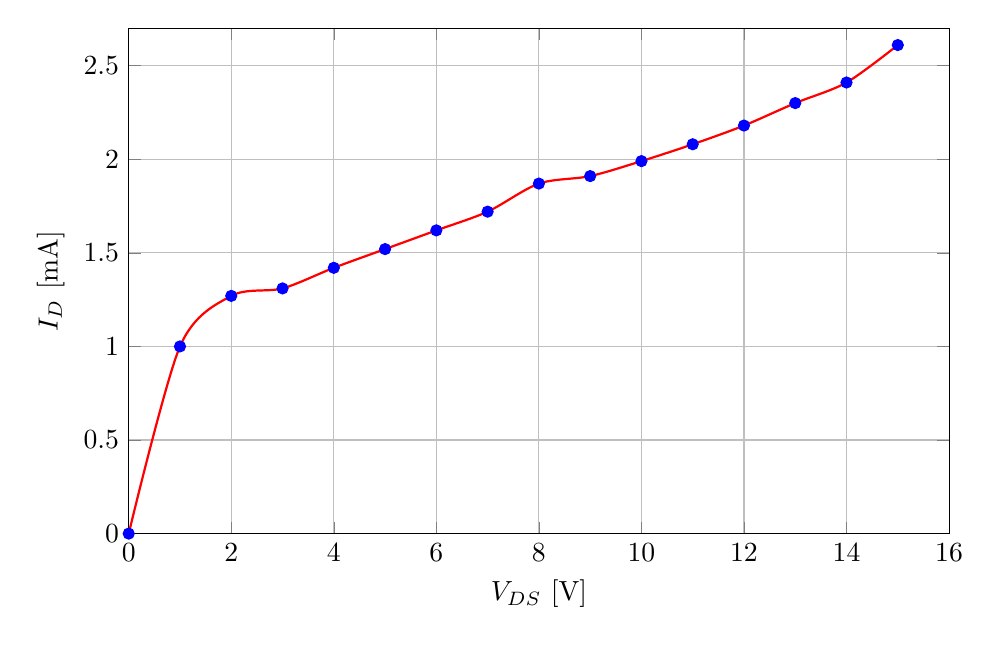
\begin{tikzpicture}
      \begin{axis}[
        width=12cm, height=8cm,
        xlabel={$V_{DS}$ [V]},
        ylabel={$I_{D}$ [mA]},
        legend style={at={(0.5,-0.2)},anchor=north,legend columns=2},
        grid=both,
        xmin=0, xmax=16,
        ymin=0, ymax=2.7,
      ]
        % Puntos medidos
        \addplot[
          only marks,
          mark=*,
          mark size=2pt,
          blue
        ] coordinates {
          (0,0)
          (1,1)
          (2,1.27)
          (3,1.31)
          (4,1.42)
          (5,1.52)
          (6,1.62)
          (7,1.72)
          (8,1.87)
          (9,1.91)
          (10,1.99)
          (11,2.08)
          (12,2.18)
          (13,2.30)
          (14,2.41)
          (15,2.61)
        };
    
        % Curva suavizada
        \addplot[
          smooth,
          thick,
          red
        ] coordinates {
          (0,0)
          (1,1)
          (2,1.27)
          (3,1.31)
          (4,1.42)
          (5,1.52)
          (6,1.62)
          (7,1.72)
          (8,1.87)
          (9,1.91)
          (10,1.99)
          (11,2.08)
          (12,2.18)
          (13,2.30)
          (14,2.41)
          (15,2.61)
        };
      \end{axis}
    \end{tikzpicture}
    }
    \caption{Curva $I_D = f(V_{DS})$ obtenida experimentalmente.}
\end{figure}


\chapter{Estrangulamiento del canal}
    \section{Actividad de simulación}
    \begin{figure}[ht!]
        \centering
        \includegraphics[width=1\linewidth]{pictures/estrangulamiento.png}
        \caption{circuito simulado en LTSpice.}
    \end{figure}
    
    \begin{figure}[ht!]
        \centering
        \includegraphics[width=0.9\linewidth]{pictures/graf-estrangulamiento.png}
        \caption{gráfica de simulación $I_D = f(V_{GS})$}
    \end{figure}

Se puede observar en la gráfica obtenida de la simulación que $V_{GS_{(off)}} = -1.4V$ e
$I_{DSS} \approx 2.1mA $, lo que se corresponde con la gráfica de la figura \ref{fig:graf-saturacion} 
y la hoja de datos, en la cual se tiene la siguiente información:

\begin{table}[h!]
    \centering
    \begin{tabular}{|c| c c c |c|}
        \hline
        Symbol & Min & Typ & Max & Unit\\
        \hline
        $V_{GS_{(off)}}$ & -0.5 & -  & -7 & Vdc    \\
        \hline
    \end{tabular}
    \caption{magnitud de $V_{GS_{(off)}}$ sacado del datasheet.}
\end{table}

\section{Actividad de laboratorio}
\begin{table}[h!]
    \centering
    \begin{minipage}{0.45\linewidth}
        \centering
        \begin{tabular}{c c}
            \toprule
            $V_{GS}$ [V] & $I_{DS}$ [mA] \\
            \midrule
            0    & 1.54  \\
            -0.1 & 0.98  \\
            -0.2 & 0.32  \\
            -0.3 & 0.03  \\
            -0.4 & 0.003 \\
            \bottomrule
        \end{tabular}
    \end{minipage}%
    \hspace{0.05\linewidth}
    \begin{minipage}{0.45\linewidth}
        \centering
        \begin{tabular}{c c}
            \toprule
            $V_{GS}$ [V] & $I_{DS}$ [mA] \\
            \midrule
            -0.5 & 0     \\
            -0.6 & 0     \\
            -0.7 & 0     \\
            -0.8 & 0     \\
            -0.9 & 0     \\
            -1.0 & 0     \\
            \bottomrule
        \end{tabular}
    \end{minipage}
    \caption{Valores de $I_{DS}$ en función de $V_{GS}$ para $V_{DS}=10$ V.}
\end{table}


\begin{figure}[h!]
\centering
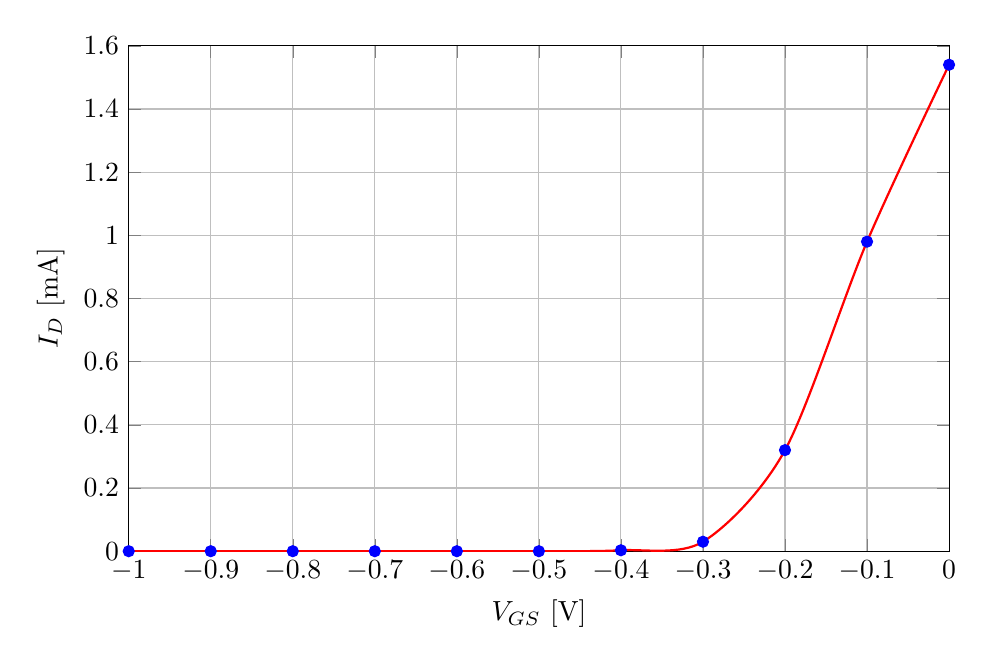
\begin{tikzpicture}
  \begin{axis}[
    width=12cm, height=8cm,
    xlabel={$V_{GS}$ [V]},
    ylabel={$I_{D}$ [mA]},
    legend style={at={(0.5,-0.2)},anchor=north,legend columns=3},
    grid=both,
    xmin=-1, xmax=0,
    ymin=0, ymax=1.6,
  ]
    % Puntos experimentales
    \addplot[
      only marks,
      mark=*,
      mark size=2pt,
      blue
    ] coordinates {
      (0,1.54)
      (-0.1,0.98)
      (-0.2,0.32)
      (-0.3,0.03)
      (-0.4,0.003)
      (-0.5,0)
      (-0.6,0)
      (-0.7,0)
      (-0.8,0)
      (-0.9,0)
      (-1.0,0)
    };

    % Curva suavizada
    \addplot[
      smooth,
      thick,
      red
    ] coordinates {
      (0,1.54)
      (-0.1,0.98)
      (-0.2,0.32)
      (-0.3,0.03)
      (-0.4,0.003)
      (-0.5,0)
      (-0.6,0)
      (-0.7,0)
      (-0.8,0)
      (-0.9,0)
      (-1.0,0)
    };
  \end{axis}
\end{tikzpicture}
\caption{Curva $I_D = f(V_{GS})$ obtenida de datos experimentales}
\end{figure}

\chapter{Característica de transferencia universal}
\section{Actividad de simulación}
\begin{figure}[ht!]
    \centering
    \includegraphics[width=1\linewidth]{pictures/curva-trans-universal.png}
    \caption{circuito simulado en LTSpice.}
\end{figure}

\begin{figure}[ht!]
    \centering
    \includegraphics[width=0.9\linewidth]{pictures/graf-curva-trans-universal.png}
    \caption{gráfica $I_D = f(V_{GS})$.}
\end{figure}

\section{Actividad de laboratorio}

\begin{table}[h!]
    \centering
    \small
    \begin{tabular}{|c| ccccccccc|}
        \hline
        & \multicolumn{9}{c|}{$I_{DS}$ [mA]} \\
        \hline
        $V_{GS}$ [V] & $V_{DS}=0$ & $0.05$ & $0.10$ & $0.20$ & $0.50$ & $1.00$ & $2.00$ & $5.00$ & $10.00$ \\
        \hline
        0     & 0.000  & 0.238  & 0.476  & 0.952  & 2.001  & 2.006  & 2.016  & 2.046  & 2.096  \\
        -0.1  & 0.000  & 0.181  & 0.362  & 0.725  & 1.161  & 1.164  & 1.170  & 1.187  & 1.217  \\
        -0.2  & 0.000  & 0.125  & 0.249  & 0.499  & 0.550  & 0.551  & 0.554  & 0.562  & 0.576  \\
        -0.3  & 0.000  & 0.068  & 0.136  & 0.163  & 0.1633 & 0.1637 & 0.1645 & 0.1670 & 0.1710 \\
        -0.35 & 0.000  & 0.040  & 0.0556 & 0.0556 & 0.0557 & 0.0559 & 0.0562 & 0.0570 & 0.0583 \\
        -0.4  & 0.000  & 0.0045 & 0.0045 & 0.0045 & 0.00455& 0.00456& 0.00458& 0.00465& 0.00476 \\
        \hline
    \end{tabular}
    \caption{Tabla de $I_{DS} = f(V_{GS})$ para distintos valores de $V_{DS}$.}
\end{table}


\begin{figure}[h!]
\centering
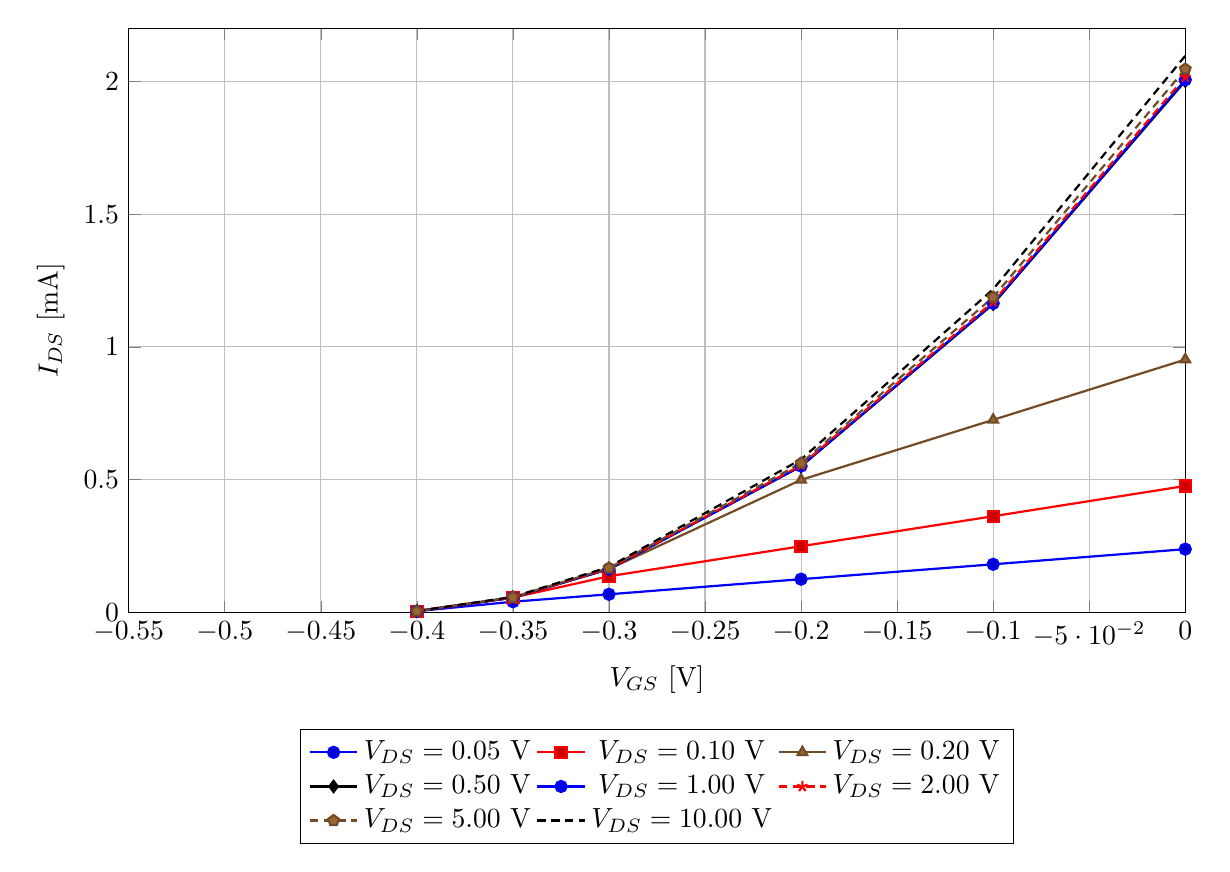
\begin{tikzpicture}
\begin{axis}[
    width=15cm, height=9cm,
    xlabel={$V_{GS}$ [V]},
    ylabel={$I_{DS}$ [mA]},
    legend style={at={(0.5,-0.2)},anchor=north,legend columns=3},
    grid=both,
    xmin=-0.55, xmax=0,
    ymin=0, ymax=2.2,
]

% VDS = 0.05 V
\addplot+[thick,mark=*] table {
VGS IDS
0.00   0.238
-0.1   0.181
-0.2   0.125
-0.3   0.068
-0.35  0.040
-0.4   0.0045
};
\addlegendentry{$V_{DS}=0.05$ V}

% VDS = 0.10 V
\addplot+[thick,mark=square*] table {
VGS IDS
0.00   0.476
-0.1   0.362
-0.2   0.249
-0.3   0.136
-0.35  0.0556
-0.4   0.0045
};
\addlegendentry{$V_{DS}=0.10$ V}

% VDS = 0.20 V
\addplot+[thick,mark=triangle*] table {
VGS IDS
0.00   0.952
-0.1   0.725
-0.2   0.499
-0.3   0.163
-0.35  0.0556
-0.4   0.0045
};
\addlegendentry{$V_{DS}=0.20$ V}

% VDS = 0.50 V
\addplot+[thick,mark=diamond*] table {
VGS IDS
0.00   2.001
-0.1   1.161
-0.2   0.550
-0.3   0.1633
-0.35  0.0557
-0.4   0.00455
};
\addlegendentry{$V_{DS}=0.50$ V}

% VDS = 1.00 V
\addplot+[thick,mark=otimes*] table {
VGS IDS
0.00   2.006
-0.1   1.164
-0.2   0.551
-0.3   0.1637
-0.35  0.0559
-0.4   0.00456
};
\addlegendentry{$V_{DS}=1.00$ V}

% VDS = 2.00 V
\addplot+[thick,mark=star] table {
VGS IDS
0.00   2.016
-0.1   1.170
-0.2   0.554
-0.3   0.1645
-0.35  0.0562
-0.4   0.00458
};
\addlegendentry{$V_{DS}=2.00$ V}

% VDS = 5.00 V
\addplot+[thick,mark=pentagon*] table {
VGS IDS
0.00   2.046
-0.1   1.187
-0.2   0.562
-0.3   0.1670
-0.35  0.0570
-0.4   0.00465
};
\addlegendentry{$V_{DS}=5.00$ V}

% VDS = 10.00 V
\addplot+[thick,mark=Mercedes star*] table {
VGS IDS
0.00   2.096
-0.1   1.217
-0.2   0.576
-0.3   0.1710
-0.35  0.0583
-0.4   0.00476
};
\addlegendentry{$V_{DS}=10.00$ V}

\end{axis}
\end{tikzpicture}
\caption{Curvas $I_{DS}$ vs $V_{GS}$ para distintos valores de $V_{DS}$ (JFET 2N5457, datos aproximados).}
\end{figure}


\chapter{Característica de salida}
    \section{Actividad de simulación}
    \begin{figure}[ht!]
        \centering
        \includegraphics[width=1\linewidth]{pictures/caract-salida.png}
        \caption{circuito simulado en LTSpice.}
    \end{figure}
    
    \begin{figure}[ht!]
        \centering
        \includegraphics[width=0.9\linewidth]{pictures/graf-caract-salida.png}
        \caption{curvas de salida obtenidas de simulación. Gráfica $I_D = f(V_{DS})$}
    \end{figure}
    
    \section{Actividad de laboratorio}
    \begin{table}[h!]
    \centering
    \begin{tabular}{|c| cccc|}
    \hline
     & \multicolumn{4}{c|}{$I_{DS}$ [mA]} \\
    \hline
    $V_{DS}$ [V] & $V_{GS}=0V$ & $V_{GS}=-0.1V$ & $V_{GS}=-0.2V$ & $V_{GS}=-0.3V$ \\
    \hline
    0  & 0    & 0     & 0     & 0   \\
    1  & 0.84 & 0.32  & 0.05  & 0.0026 \\
    2  & 0.98 & 0.39  & 0.07  & 0.0043 \\
    3  & 1.10 & 0.46  & 0.09  & 0.0061 \\
    4  & 1.24 & 0.52  & 0.12  & 0.0085 \\
    5  & 1.37 & 0.57  & 0.132 & 0.0107 \\
    6  & 1.29 & 0.62  & 0.155 & 0.0123 \\
    7  & 1.47 & 0.67  & 0.172 & 0.0155 \\
    8  & 1.54 & 0.73  & 0.196 & 0.0183 \\
    9  & 1.64 & 0.77  & 0.212 & 0.0215 \\
    10 & 1.72 & 0.83  & 0.212 & 0.0255 \\
    \hline
    \end{tabular}
    \caption{Valores de $I_{DS}$ en función de $V_{DS}$ para distintos $V_{GS}$.}
    \end{table}
    
    \begin{figure}[h!]
\centering
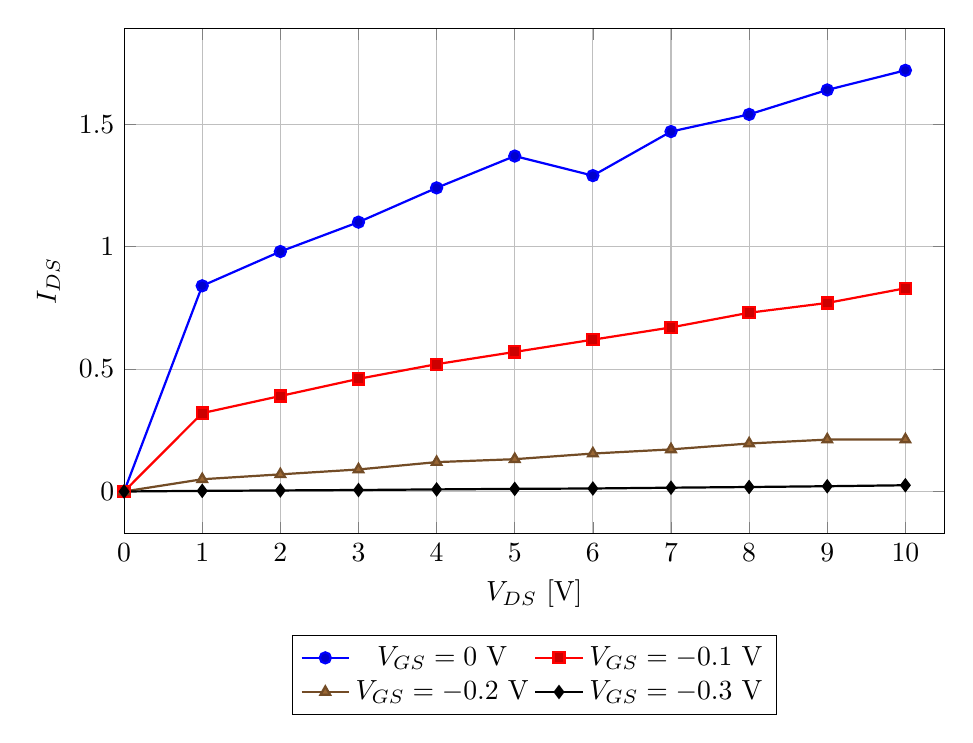
\begin{tikzpicture}
\begin{axis}[
    width=12cm, height=8cm,
    xlabel={$V_{DS}$ [V]},
    ylabel={$I_{DS}$},
    legend style={at={(0.5,-0.2)},anchor=north,legend columns=2},
    grid=both,
    xmin=0, xmax=10.5,
]

% VGS = 0 V
\addplot+[thick,mark=*] table {
VDS IDS
0  0
1  0.84
2  0.98
3  1.10
4  1.24
5  1.37
6  1.29
7  1.47
8  1.54
9  1.64
10 1.72
};
\addlegendentry{$V_{GS}=0$ V}

% VGS = -0.1 V
\addplot+[thick,mark=square*] table {
VDS IDS
0  0
1  0.32
2  0.39
3  0.46
4  0.52
5  0.57
6  0.62
7  0.67
8  0.73
9  0.77
10 0.83
};
\addlegendentry{$V_{GS}=-0.1$ V}

% VGS = -0.2 V
\addplot+[thick,mark=triangle*] table {
VDS IDS
0  0
1  0.05
2  0.07
3  0.09
4  0.12
5  0.132
6  0.155
7  0.172
8  0.196
9  0.212
10 0.212
};
\addlegendentry{$V_{GS}=-0.2$ V}

% VGS = -0.3 V (µA)
\addplot+[thick,mark=diamond*] table {
VDS IDS
0  0
1  0.0026
2  0.0043
3  0.0061
4  0.0085
5  0.0107
6  0.0123
7  0.0155
8  0.0183
9  0.0215
10 0.0255
};
\addlegendentry{$V_{GS}=-0.3$ V}
\end{axis}
\end{tikzpicture}
\caption{Curvas $I_{DS}$ vs $V_{DS}$ para distintos valores de $V_{GS}$, según la tabla experimental.}
\end{figure}

\chapter{Interpretación de hoja de datos}

\begin{table}[h!]
\centering
\small
\begin{tabular}{l c c c c l}
\toprule
Parámetro & Símbolo & Condición & Mín & Típ & Máx \\
\midrule
Corriente de saturación drenaje & $I_{DSS}$ & $V_{DS}=15$ V,\ $V_{GS}=0$ & 1.0 & 3.0 & 5.0 mA \\
Tensión drenaje–source máx & $V_{DS}$ & rating absoluto & \multicolumn{3}{c}{25 V} \\
Tensión gate–source máx (inversa) & $V_{GS}$ & rating absoluto & \multicolumn{3}{c}{-25 V} \\
Potencia disipada @25 °C & $P_{D}$ & TO-92,\ $T_A=25^\circ$C & \multicolumn{3}{c}{310 mW} \\
Derating térmico &  &  & \multicolumn{3}{c}{2.82 mW/°C} \\
Tensión ruptura G–S & $V_{(BR)GSS}$ & $I_G=-10\,\mu$A,\ $V_{DS}=0$ & -25 & — & — V \\
Tensión de corte gate–source & $V_{GS(\text{off})}$ & $V_{DS}=15$ V,\ $I_D=10$ nA & -0.5 & — & -6.0 V \\
Tensión $V_{GS}$ a $I_D=100\,\mu$A & $V_{GS}$ & $V_{DS}=15$ V & — & -2.5 & — V \\
\bottomrule
\end{tabular}
\caption{Especificaciones eléctricas típicas del JFET 2N5457 a $25^\circ$C (según hoja de datos).}
\end{table}

\section*{Explicación de los parámetros}

\begin{itemize}
  \item \textbf{Corriente de saturación drenaje ($I_{DSS}$):} es la corriente máxima de drenaje cuando la compuerta está a 0 V respecto a la fuente. Indica la capacidad de conducción del canal cuando está totalmente abierto.
  
  \item \textbf{Tensión drenaje–source máx ($V_{DS}$):} valor máximo de tensión permitido entre drenaje y fuente. Superarlo puede dañar permanentemente el dispositivo.
  
  \item \textbf{Tensión gate–source máx ($V_{GS}$):} tensión máxima en polarización inversa entre compuerta y fuente. Su función es proteger la juntura P–N de la compuerta.
  
  \item \textbf{Potencia disipada ($P_{D}$):} máxima potencia que el dispositivo puede disipar en forma de calor a temperatura ambiente de 25 °C.
  
  \item \textbf{Derating térmico:} factor que indica cuánto debe reducirse la potencia disipada máxima por cada grado que aumenta la temperatura ambiente por encima de 25 °C.
  
  \item \textbf{Tensión de ruptura G–S ($V_{(BR)GSS}$):} tensión de ruptura de la juntura gate–source. Marca el límite a partir del cual la compuerta comienza a conducir corriente de manera destructiva.
  
  \item \textbf{Tensión de corte gate–source ($V_{GS(\text{off})}$):} tensión de compuerta negativa en la que el canal se cierra y la corriente de drenaje se reduce prácticamente a cero. Este parámetro define el rango de control del JFET.
  
  \item \textbf{Tensión $V_{GS}$ a $I_D=100\,\mu$A:} valor típico de compuerta que establece una corriente de drenaje de referencia. Se utiliza para comparar dispositivos y verificar su rango de operación.
\end{itemize}

\noindent



\chapter{Conclusión}

El presente trabajo práctico permitió comprender en detalle las capacidades y limitaciones de los transistores JFET, así como también obtener una visión más clara de las aplicaciones en las que este tipo de dispositivo puede ser utilizado. A partir de las mediciones realizadas y de la consulta de la hoja de datos, se logró contrastar la teoría con la práctica y afianzar conceptos fundamentales de la electrónica de dispositivos.  

En cuanto a la medición de parámetros y a la interpretación de la hoja de datos, no se presentaron mayores dificultades. Sin embargo, el principal desafío encontrado fue la disponibilidad del componente: debido a la escasez y a la tendencia hacia la obsolescencia de los JFET, resultó complejo conseguir un ejemplar que funcionara adecuadamente. El mercado electrónico local presenta limitaciones en este aspecto, lo que obligó a probar diferentes modelos hasta dar con uno que cumpliera, al menos de manera aproximada, con las características especificadas en su hoja de datos.  

En síntesis, la experiencia resultó enriquecedora no solo por el análisis técnico, sino también porque puso en evidencia las restricciones prácticas vinculadas a la disponibilidad de componentes en el entorno real.

Se adjunta el datasheet del dispositivo utilizado:

\includepdf[pages=1-2]{2N5457.PDF}


\end{document}
